% Version  Date        Author            Notes
% 1        ?           Tobias Lutz
% 2        April 2016  Tasnad Kernetzky  Updated to new IEEEtran class (v. 1.8)
%
%
\documentclass[journal, a4paper]{IEEEtran}

% check if we are running lua(la)tex and load font related packages appropriately
\usepackage{ifluatex}
\ifluatex
    \usepackage{fontspec}
\else
    \usepackage[T1]{fontenc}
    \usepackage[utf8]{inputenc}
\fi

% some very useful LaTeX packages include:
%\usepackage{cite}      % Written by Donald Arseneau
                        % V1.6 and later of IEEEtran pre-defines the format
                        % of the cite.sty package \cite{} output to follow
                        % that of IEEE. Loading the cite package will
                        % result in citation numbers being automatically
                        % sorted and properly "ranged". i.e.,
                        % [1], [9], [2], [7], [5], [6]
                        % (without using cite.sty)
                        % will become:
                        % [1], [2], [5]--[7], [9] (using cite.sty)
                        % cite.sty's \cite will automatically add leading
                        % space, if needed. Use cite.sty's noadjust option
                        % (cite.sty V3.8 and later) if you want to turn this
                        % off. cite.sty is already installed on most LaTeX
                        % systems. The latest version can be obtained at:
                        % http://www.ctan.org/tex-archive/macros/latex/contrib/supported/cite/

\usepackage{graphicx}   % Written by David Carlisle and Sebastian Rahtz
                        % Required if you want graphics, photos, etc.
                        % graphicx.sty is already installed on most LaTeX
                        % systems. The latest version and documentation can
                        % be obtained at:
                        % http://www.ctan.org/tex-archive/macros/latex/required/graphics/
                        % Another good source of documentation is "Using
                        % Imported Graphics in LaTeX2e" by Keith Reckdahl
                        % which can be found as esplatex.ps and epslatex.pdf
                        % at: http://www.ctan.org/tex-archive/info/

%\usepackage{psfrag}    % Written by Craig Barratt, Michael C. Grant,
                        % and David Carlisle
                        % This package allows you to substitute LaTeX
                        % commands for text in imported EPS graphic files.
                        % In this way, LaTeX symbols can be placed into
                        % graphics that have been generated by other
                        % applications. You must use latex->dvips->ps2pdf
                        % workflow (not direct pdf output from pdflatex) if
                        % you wish to use this capability because it works
                        % via some PostScript tricks. Alternatively, the
                        % graphics could be processed as separate files via
                        % psfrag and dvips, then converted to PDF for
                        % inclusion in the main file which uses pdflatex.
                        % Docs are in "The PSfrag System" by Michael C. Grant
                        % and David Carlisle. There is also some information
                        % about using psfrag in "Using Imported Graphics in
                        % LaTeX2e" by Keith Reckdahl which documents the
                        % graphicx package (see above). The psfrag package
                        % and documentation can be obtained at:
                        % http://www.ctan.org/tex-archive/macros/latex/contrib/supported/psfrag/

%\usepackage{subfigure} % Written by Steven Douglas Cochran
                        % This package makes it easy to put subfigures
                        % in your figures. i.e., "figure 1a and 1b"
                        % Docs are in "Using Imported Graphics in LaTeX2e"
                        % by Keith Reckdahl which also documents the graphicx
                        % package (see above). subfigure.sty is already
                        % installed on most LaTeX systems. The latest version
                        % and documentation can be obtained at:
                        % http://www.ctan.org/tex-archive/macros/latex/contrib/supported/subfigure/

%\usepackage{url}       % Written by Donald Arseneau
                        % Provides better support for handling and breaking
                        % URLs. url.sty is already installed on most LaTeX
                        % systems. The latest version can be obtained at:
                        % http://www.ctan.org/tex-archive/macros/latex/contrib/other/misc/
                        % Read the url.sty source comments for usage information.

%\usepackage{stfloats}  % Written by Sigitas Tolusis
                        % Gives LaTeX2e the ability to do double column
                        % floats at the bottom of the page as well as the top.
                        % (e.g., "\begin{figure*}[!b]" is not normally
                        % possible in LaTeX2e). This is an invasive package
                        % which rewrites many portions of the LaTeX2e output
                        % routines. It may not work with other packages that
                        % modify the LaTeX2e output routine and/or with other
                        % versions of LaTeX. The latest version and
                        % documentation can be obtained at:
                        % http://www.ctan.org/tex-archive/macros/latex/contrib/supported/sttools/
                        % Documentation is contained in the stfloats.sty
                        % comments as well as in the presfull.pdf file.
                        % Do not use the stfloats baselinefloat ability as
                        % IEEE does not allow \baselineskip to stretch.
                        % Authors submitting work to the IEEE should note
                        % that IEEE rarely uses double column equations and
                        % that authors should try to avoid such use.
                        % Do not be tempted to use the cuted.sty or
                        % midfloat.sty package (by the same author) as IEEE
                        % does not format its papers in such ways.

%\usepackage{amsmath}   % From the American Mathematical Society
                        % A popular package that provides many helpful commands
                        % for dealing with mathematics. Note that the AMSmath
                        % package sets \interdisplaylinepenalty to 10000 thus
                        % preventing page breaks from occurring within multiline
                        % equations. Use:
%\interdisplaylinepenalty=2500
                        % after loading amsmath to restore such page breaks
                        % as IEEEtran.cls normally does. amsmath.sty is already
                        % installed on most LaTeX systems. The latest version
                        % and documentation can be obtained at:
                        % http://www.ctan.org/tex-archive/macros/latex/required/amslatex/math/



% Other popular packages for formatting tables and equations include:

%\usepackage{array}
% Frank Mittelbach's and David Carlisle's array.sty which improves the
% LaTeX2e array and tabular environments to provide better appearances and
% additional user controls. array.sty is already installed on most systems.
% The latest version and documentation can be obtained at:
% http://www.ctan.org/tex-archive/macros/latex/required/tools/

% V1.6 of IEEEtran contains the IEEEeqnarray family of commands that can
% be used to generate multiline equations as well as matrices, tables, etc.

% Also of notable interest:
% Scott Pakin's eqparbox package for creating (automatically sized) equal
% width boxes. Available:
% http://www.ctan.org/tex-archive/macros/latex/contrib/supported/eqparbox/

% *** Do not adjust lengths that control margins, column widths, etc. ***
% *** Do not use packages that alter fonts (such as pslatex).         ***
% There should be no need to do such things with IEEEtran.cls V1.6 and later.


% Your document starts here!
\begin{document}

% Define document title and author
\title{Authentication based on DRAM PUFs}
\author{Chirag Mahaveer Parmar
\thanks{Advisor: Hedongliang Liu, Associate Professorship of Coding and Cryptography}}
\markboth{Seminar in Coding and Cryptography}{}
\maketitle

% Write abstract here
\begin{abstract}
The short abstract (50-80 words) is intended to give the reader an overview of the work.
Keep in mind that he does not known the work yet.
\end{abstract}

% Each section begins with a \section{title} command
\section{Introduction}
% \IEEEPARstart{}{} creates a tall first letter for this first paragraph
\IEEEPARstart{I}{n} In light of the IoT era the world has seen a spike in the number of smart devices deployed in the market. These ubiquitous smart devices can be found anywhere, from toasters to cars. While they bring a lot of advantages to the table they add a profound amount of concern regarding security and privacy. The most prominent security concern includes counterfeit or tampered hardware. [cite dem all]

Mitigating these security risks requires hardware-intrinsic security mechanisms that support authentication and identification of the device. A known solution requires cryptographic keys to be burned in at manufacturing time and then later used in symmetric/asymmetric protocols for authentication. Although this approach is susceptible to key extraction attacks giving way to cloning. Thus, Physically Unclonable Functions have been proposed as a solution to this issue.

PUFs by definition are unclonable and also because they exploit the process variations of manufacturing to form a hardware-based fingerprint. This hardware based fingerprint with a supporting lightweight protocol can then be used for authentication. Clearly, it is very important for the PUF instance to be intrinsic to the hardware that needs to be authenticated. The intrinsic nature can be assured either by addition of dedicated circuits or by using PUFs inherent to the device. Since the latter adds costs to the manufacturing process, inherent and intrinsic PUFs are much preferred. DRAM based PUFs are such a class of PUFs, because they can be found in almost all COTS devices.

This paper briefly touches on the basics of PUFs and dives into how DRAMs are used as PUF instances in the Theory section. Through means of survey it presents different types of authentication mechanisms used in conjunction with DRAM based PUFs ([add section details here]). Finally, it also presents the main implementation objectives accompanied by a summary of metrics by means of survey.

\section{Theory}
This sections goes into the basics of PUFs and workings of DRAM PUFs.

\subsection{PUFs}
In practice most PUFs are characterized by challenges and responses. A challenge is the input given to the PUF, which then utilizes the random manufacturing process variations to convert the challenge to a response. The randomness makes the response unpredictable and because these variations cannot be controlled, even by the manufacturer, the response is unclonable on any other device. Hence, the response can be used as a hardware intrinsic fingerprint for authentication.

\begin{figure}[!hbt]
    % Center the figure.
    \begin{center}
    % Include the eps file, scale it such that it's width equals the column width. You can also put width=8cm for example...
    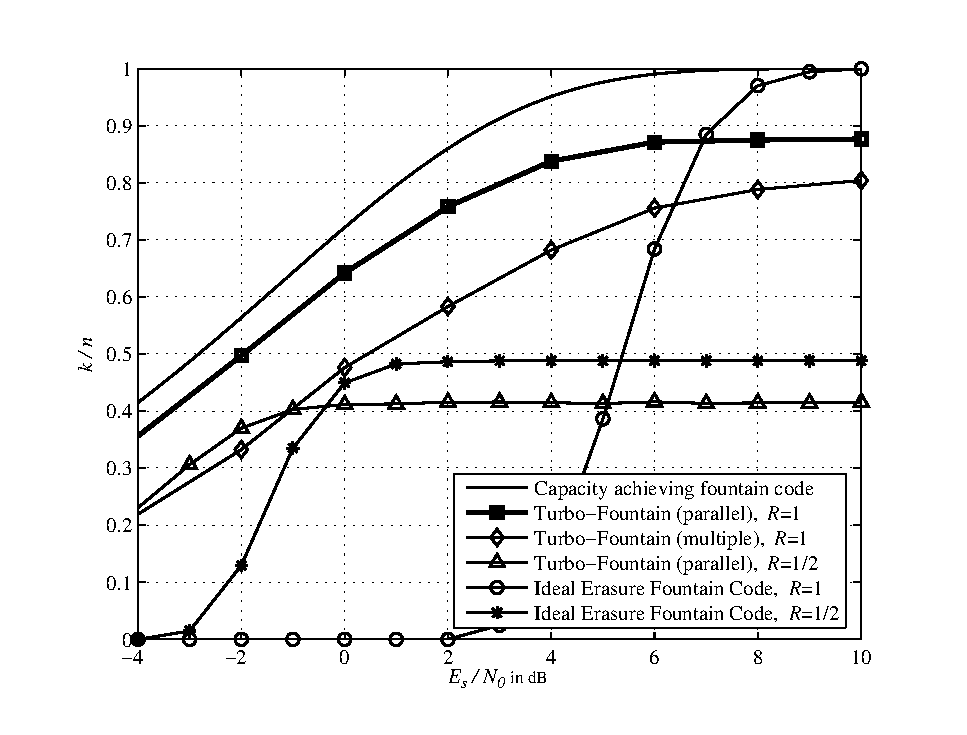
\includegraphics[width=\columnwidth]{figs/plot_tf.eps}
    % Create a subtitle for the figure.
    \caption{PUFS}
    % Define the label of the figure. It's good to use 'fig:title', so you know that the label belongs to a figure.
    \label{fig:tf_plot}
    \end{center}
\end{figure}

PUFs are mainly categorized into strong PUFs and weak PUFs based on the number of unique challenge response pairs (CRPs) they can generate. Larger the CRP database, the stronger the PUF. Both kinds of PUFs have appropriate supporting authentication protocols as discussed in the next sections.

\subsection{DRAM PUFs}
There are different methods in which the process variations of DRAM can be leveraged and they are explained below:

\textbf{Startup:} In this method, the startup state of the DRAM is used for unique fingerprinting. As mentioned in [tehranipoor] “DRAMs have seemingly random startup values”. This is because the bitlines on DRAM are precharged to vdd/2 which makes the sense amplifier equally likely to read a ‘1’ or ‘0’. But, due to the process variations of manufacturing most bits have either a bias towards a ‘1’ or a ‘0’. Hence, the startup values of the DRAM are randomized by the random process variations. It is noted though that some bits have a neutral skew/bias i.e. they randomly switch to ‘1’ or ‘0’ over multiple startups. These bits can be used for random number generation. This method is not suitable for authentication using the traditional CRP database approach, because startup values cannot be varied by writing the challenge to memory before startup.

\textbf{Write Failures:} In this method, process variations affecting the write reliability are exploited. Under normal operation, the write enable signal activates the bit lines i.e. connects them to the data bus which then overrides the bit line voltage. As a result, the DRAM cells would be overwritten by the value on the data bus. For normal operation the duty cycle of the write signal is chosen such that all DRAM cells can successfully. But for PUF operation, the duty cycle is deliberately reduced which results in some DRAM cells being overwritten while others are not. If a cell has been overwritten or not depends on the manufacturing variations. The data written under PUF operation can be treated as the challenge and a subsequent read reveals the response affected by the variations.

\textbf{Refresh Pause:} In this method, the refresh of the DRAM cells is paused to allow random decaying of the data stored in memory[cite all known papers]. For normal operation DRAM cells need to be refreshed i.e. the capacitors holding the charges need to be recharged due to leakage in the circuit. If the refresh is delayed some DRAM cells decay and thereby introduce a bit flip in the stored data. Under such operation, the DRAM can be used as a PUF where the data stored before the delaying refresh can be treated as the challenge and the one after the delay as the response. An alternate method exploits data remanence properties [cite remanence from tehranipoor] of the DRAM, where the DRAM is completely switched off and then the cells are read.

\section{Implementation Objectives}
In order to analyse the various presented methods measurements have to be made. Almost all surveyed papers use either hamming distance and fractional hamming distance or jaccard index [cite jaccard index] for measuring the properties of the PUFs. The usage of one over the other is debatable although [cite Xiong et al.] claims jaccard index to be a better metric because it takes into consideration only the bits that flip as opposed to fractional hamming distance which weighs all bits of the CRP equally. 

[insert formulas for both and properties too o jaccard index vs 1 jaccard index]

\textit{Uniqueness.} Uniqueness in PUFs is measured by comparing responses for the same challenges on different PUF instances. Greater difference in responses indicates stronger uniqueness.  The comparison is measured using either hamming distance(needs to be high) or the jaccard index(needs to be low). All surveyed work proves the uniqueness through experimentation on PUF instances of different DRAM modules, sutar et al. goes a step further to analyze the uniqueness of different PUF instances within the same DRAM module. Since the experiment conducted by sutar et al. sparks interest the table below summarizes their results.

% This is how you define a table: the [!hbt] means that LaTeX is forced (by the !) to place the table exactly here (by h), or if that doesnt work because of a pagebreak or so, it tries to place the table to the bottom of the page (by b) or the top (by t).
\begin{table}[!hbt]
    % Center the table
    \begin{center}
    % Title of the table
    \caption{Simulation Parameters}
    \label{tab:simParameters}
    % Table itself: here we have two columns which are centered and have lines to the left, right and in the middle: |c|c|
    \begin{tabular}{|c|c|}
        % To create a horizontal line, type \hline
        \hline
        % To end a column type &
        % For a linebreak type \\
        Information message length & $k=16000$ bit \\
        \hline
        Radio segment size & $b=160$ bit \\
        \hline
        Rate of component codes & $R_{cc}=1/3$\\
        \hline
        Polynomial of component encoders & $[1 , 33/37 , 25/37]_8$\\
        \hline
    \end{tabular}
    \end{center}
\end{table}

\textit{Robustness.} Robustness of a PUF is measured by comparing the responses for the same challenges on the same PUF instances but on consequent executions. Hence robustness, in this context can also be seen as \textbf{reproducibility}. For robustness we need the HD to be close to 0 and the jaccard index to be close to 1. These measurements of robustness (same PUF instances) are further compared to the measurements of uniqueness (different PUF instances) to show \textbf{separability} or non-existence of false positives.

Robustness is also measured against temperature variations and aging. Almost all research work reports a drop in reproducibility as the temperature is increased. Although this drop is inferred differently in different conducted research. [hashemian et al.] which uses write failures for PUF operation claims the temperature induced variability to be not too profound thereby proving stability. [Xiong et al.] which uses the refresh pause approach makes a relation between the temperature variation and decay rate and claims that the decay characteristics are unaffected. [Xiong et al], for the above relation, suggests decreasing the refresh pause interval under increased temperature conditions. [Sutar et al] recommend adequate error correction and use dynamic thresholds (depending on temperature) . Aging effects on PUFs robustness is found to be negligible by most research papers.

\textit{Run-time Access.} Based on the methods DRAM PUFs are limited in access. For run-time access of DRAM PUFs it is important that the PUF operation doesn’t hinder the functioning of the OS and applications. The solution presented by [tehranipoor] restricts the access to the DRAM PUF to an early boot stage because DRAM startup values cannot be accessed later. Whereas, write failures based DRAM PUFs offer the flexibility of run time access.

Refresh pause based  DRAM PUFs can offer run-time access but with modifications to the kernel in some cases. When LPDDR DRAM is being used the PUFs can be accessed at run-time due to “Partial Array Self-Refresh” functionality [cite liu et al. and sutar et al]. When DRAMs are split by different memory controllers they can still provide run-time access by splitting the memory per controller for OS and PUF respectively. Special case arises when the DRAM being used has none of the above features, in such case, memory ballooning[cite] is used to reserve a DRAM region and selective memory refreshing[cite] is used to refresh selected regions by initiating a read. Xiong et al. outlines and experiments this method in their work.

\section{Authentication}
Most surveyed papers use the challenge response pairs for lightweight authentication of a client/prover (C) device towards a server/verifier (S) as described below.

\textit{Adversary and threat model.} It is assumed that all network traffic between client and server is observable by attackers except during the enrollment phase. This is also known as the passive attacker model and here the attacker can observe the previous PUF measurements that were passed to the server.

\textit{Enrollment.} The flow chart in \ref{enroll} depicts the enrollment process. The enrollment phase deals with generation of the CRP database. These challenge response pairs are then either stored on a trusted secure database or distributed to verifiers in a secure manner. It has to be made sure that different verifiers receive different parts of the CRP database, otherwise one can spoof to be the device to the other.

\begin{figure}[!hbt]
    % Center the figure.
    \begin{center}
    % Include the eps file, scale it such that it's width equals the column width. You can also put width=8cm for example...
    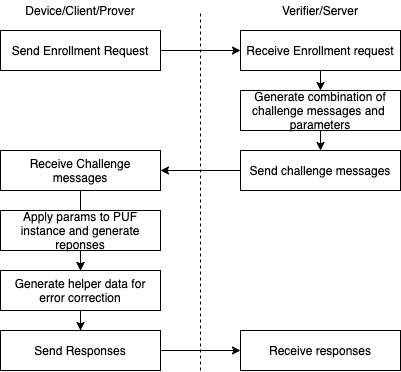
\includegraphics[width=\columnwidth]{figs/enrollment.png}
    % Create a subtitle for the figure.
    \caption{Enrollment}
    % Define the label of the figure. It's good to use 'fig:title', so you know that the label belongs to a figure.
    \label{fig:enroll}
    \end{center}
\end{figure}

\textit{One Way Authentication.} The flowchart in \ref{one_way} depicts the one-way authentication process

\begin{figure}[!hbt]
    % Center the figure.
    \begin{center}
    % Include the eps file, scale it such that it's width equals the column width. You can also put width=8cm for example...
    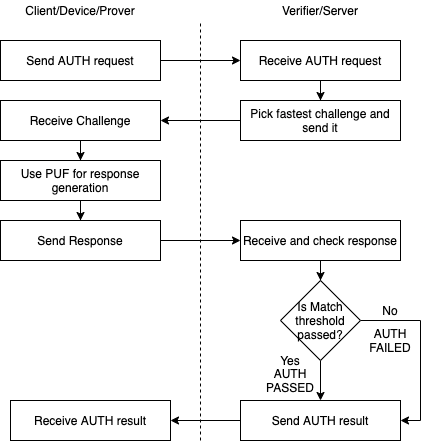
\includegraphics[width=\columnwidth]{figs/authentication.png}
    % Create a subtitle for the figure.
    \caption{1-way Authentication}
    % Define the label of the figure. It's good to use 'fig:title', so you know that the label belongs to a figure.
    \label{fig:one_way}
    \end{center}
\end{figure}

\textit{Mutual Authentication.} This is an extension of the 1-way authentication which requires storage of CRPs in form of addresses of flipped bits rather than the bit pattern itself. The device in addition to the response of flipped addresses mixes random addresses. The server verfies the device by counting the number of matched addresses and checking it against a threshold. The server then filters out the known flip addresses from the response and sends it to the device. The device verifies the server's response by matching it with its own response.

In both authentication protocols described above it is important to note that:
\begin{itemize}
    \item A CRP is never used twice. This is to prevent replay attacks. Hence a large CRP database or a strong PUF is required for continued authentication.
    \item For fast authentication it is critical to pick a CRP with the fastest possible parameters(low refresh pause interval) is picked. This requires knowledge of the PUF characteristics beforehand.
\end{itemize}

These requirements pave the way for improvements in the usage of DRAM PUFs, Parameter Reconfigurability and Characterization resp.

\textit{Parameter Variation:} Most variations in parameters and the options of reconfigurability were presented with the refresh pause method. Hence this section will focus mainly on the refresh pause method.

[Sutar et al] in their work show the reconfigurability of the refresh pause interval in order to obtain new challenge response pairs on the same PUF instance. A similar experiment is also conducted by [Xiong et al]. In both these works, the lowest refresh pause interval was 20s. After the CRPs of a particular refresh pause interval have been exhausted the interval can be increased to higher one depending on the number of “new” bit flips. Both these works also propose increasing the size of the PUF instance, in order to maintain the low refresh pause interval at the cost of DRAM space exhaustion. 

Apart from the refresh pause interval and the size of the PUF instance, [sutar et al] and [miskelly et al] demonstrate the usage of different input patterns and the effect of peripheral bits, wrapper pattern, surrounding the block of PUF instances on the response.

With these parameters at disposal, one can reconfigure the PUF instance to generate new sets of CRP pairs thereby increasing the size of the CRP database.

\textit{Characterization:} For proper usage of the reconfiguration parameters, they have to be known to the verifier beforehand so that they can be attached with the challenge message during authentication. For achieving this the DRAM module has to be characterized. In simple terms, characterization is the process of trying all kinds of combinations of parameters and observing the difference in responses[cite]. After such an exhaustive experimentation the best suitable parameters are selected and the CRP database is generated accordingly. For example, [miskelly] experiments with an all ‘0’ and all ‘1’ input pattern and selects the input pattern with a higher number of bit flips. The responses for the two are biased due to the presence of true-cells and anti-cells.

Note that characterization is assumed to take place in a trusted and secure environment. Any information leakage of the characterization parameters reveals the characteristics of the PUF and hence make them susceptible to cloning.


% Main Part
\section{Main Part}
% LaTeX takes complete care of your document layout ...
The presentation's content is summarized in the report in 4~pages.
% ... but you can insert a line break manually with two backslashes, if needed: \\
The author should fill, but not exceed, this space. \\
The report should be a self-contained report, so that it can be understood without studying additional literature.

\section{Format}
The report can be written in \LaTeX{} or Microsoft Word, but \LaTeX{} is definitely preferred.
Its appearance should be as close to this document as possible to achieve consistency in the proceedings.

% You can cite a book or paper by using \cite{reference}.
% The references will be defined at the end of this .tex file in the bibliography
References should be cited as numbers, and should be ordered by their appearance (example: ``... as shown in \cite{HOP96}, ...'').
Only references that are actually cited can be listed in the references section.
The references' format should be evident from the examples in this text.

References should be of academic character and should be published and accessible.
Your advisor can answer your questions regarding literature research.
You must cite all used sources.
Examples of good references include text books and scientific journals or conference proceedings.
If possible, citing internet pages should be avoided. In particular, Wikipedia is \emph{not} an appropriate reference in academic reports.
Avoiding references in languages other than English is recommended.

% You can reference tables and figure by using the \ref{label} command. Each table and figure needs to have a UNIQUE label.
Figures and tables should be labeled and numbered, such as in Table~\ref{tab:simParameters} and Fig.~\ref{fig:tf_plot}.

% This is how you define a table: the [!hbt] means that LaTeX is forced (by the !) to place the table exactly here (by h), or if that doesnt work because of a pagebreak or so, it tries to place the table to the bottom of the page (by b) or the top (by t).
\begin{table}[!hbt]
    % Center the table
    \begin{center}
    % Title of the table
    \caption{Simulation Parameters}
    \label{tab:simParameters}
    % Table itself: here we have two columns which are centered and have lines to the left, right and in the middle: |c|c|
    \begin{tabular}{|c|c|}
        % To create a horizontal line, type \hline
        \hline
        % To end a column type &
        % For a linebreak type \\
        Information message length & $k=16000$ bit \\
        \hline
        Radio segment size & $b=160$ bit \\
        \hline
        Rate of component codes & $R_{cc}=1/3$\\
        \hline
        Polynomial of component encoders & $[1 , 33/37 , 25/37]_8$\\
        \hline
    \end{tabular}
    \end{center}
\end{table}

% If you have questions about how to write mathematical formulas in LaTeX, please read a LaTeX book or the 'Not So Short Introduction to LaTeX': tobi.oetiker.ch/lshort/lshort.pdf

% This is how you include a eps figure in your document. LaTeX only accepts EPS or TIFF files.
\begin{figure}[!hbt]
    % Center the figure.
    \begin{center}
    % Include the eps file, scale it such that it's width equals the column width. You can also put width=8cm for example...
    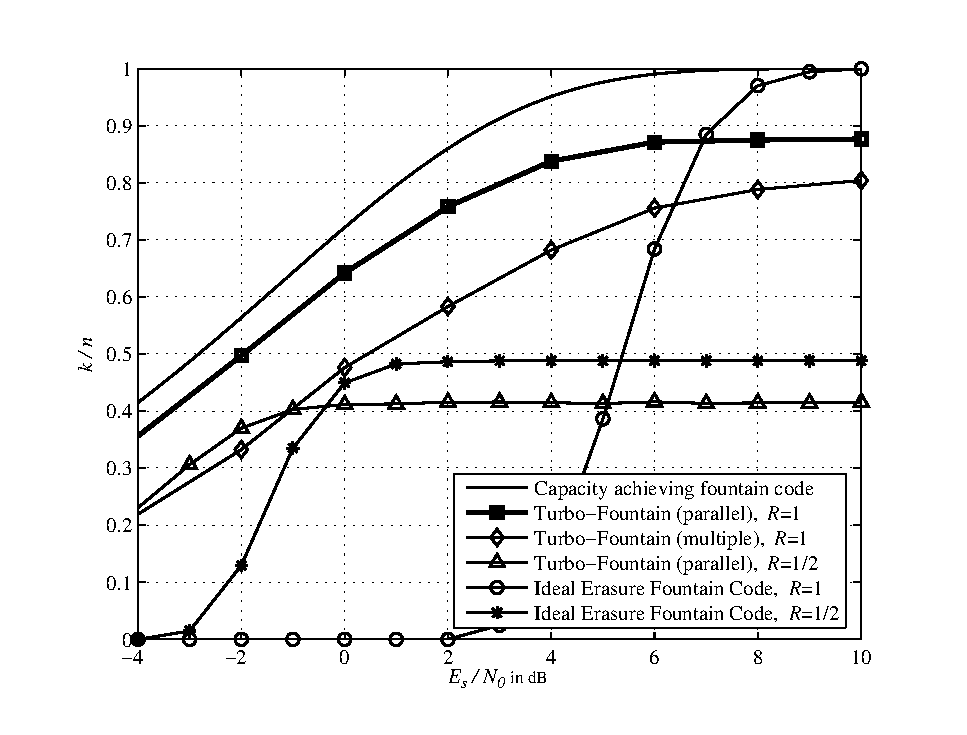
\includegraphics[width=\columnwidth]{figs/plot_tf.eps}
    % Create a subtitle for the figure.
    \caption{Simulation results on the AWGN channel. Average throughput $k/n$ vs $E_s/N_0$.}
    % Define the label of the figure. It's good to use 'fig:title', so you know that the label belongs to a figure.
    \label{fig:tf_plot}
    \end{center}
\end{figure}

\section{Filling this page}
Gallia est omnis divisa in partes tres, quarum unam incolunt Belgae, aliam Aquitani, tertiam qui ipsorum lingua Celtae, nostra Galli appellantur. Hi omnes lingua, institutis, legibus inter se differunt. Gallos ab Aquitanis Garumna flumen, a Belgis Matrona et Sequana dividit. Horum omnium fortissimi sunt Belgae, propterea quod a cultu atque humanitate provinciae longissime absunt, minimeque ad eos mercatores saepe commeant atque ea quae ad effeminandos animos pertinent important, proximique sunt Germanis, qui trans Rhenum incolunt, quibuscum continenter bellum gerunt.

\section{Conclusion}
This section summarizes the paper. Now the reader knows your work, you can go into detail a little bit more about the main aspects.


% Now we need a bibliography:
\begin{thebibliography}{1}

    %Each item starts with a \bibitem{reference} command and the details thereafter.
    \bibitem{HOP96} % Transaction paper
    J.~Hagenauer, E.~Offer, and L.~Papke. Iterative decoding of binary block
    and convolutional codes. {\em IEEE Trans. Inform. Theory},
    vol.~42, no.~2, pp.~429–-445, Mar. 1996.

    \bibitem{MJH06} % Conference paper
    T.~Mayer, H.~Jenkac, and J.~Hagenauer. Turbo base-station cooperation for intercell interference cancellation. {\em IEEE Int. Conf. Commun. (ICC)}, Istanbul, Turkey, pp.~356--361, June 2006.

    \bibitem{Proakis} % Book
    J.~G.~Proakis. {\em Digital Communications}. McGraw-Hill Book Co.,
    New York, USA, 3rd edition, 1995.

    \bibitem{talk} % Web document
    P.~N.~Edwards. How to give a talk: Changing the culture of academic public speaking.
    http://www.si.umich.edu/~pne/acadtalk.htm.

    \bibitem{5}
    IEEE Transactions \LaTeX{} and Microsoft Word Style Files.
    http://www.ieee.org/web/publications/authors/transjnl/index.html

\end{thebibliography}

% Your document ends here!
\end{document}
